% Chapter Template

\chapter{Related Work} % Main chapter title

\label{ch:02} % Change X to a consecutive number; for referencing this chapter elsewhere, use \ref{ChapterX}

Surface normal inference is a widely researched topic and can be solved in several ways. Traditionally, it can be derived from a point cloud. There are many optimization-based approaches to computing surface normals pixel-by-pixel using neighborhood information. \cite{optimized-methods} gives a comparison between some of these approaches. \cite{Holzer.S} proposed a method of using local neighbors with an interest parameter $ p $ and derives the surface normal from the eigenvectors of the corresponding covariance matrix. These approaches work well for dense input data based on a well-chosen window size.
However, in many practical datasets such as NYU Depth Dataset V2 \cite{nyu} and KITTI-Depth\cite{kitti-depth}, the point clouds are often converted from depth maps.
But the depth maps are usually very noisy and contains many missing pixels and holes in dark, shiny, or transparent areas. This poses more of a challenge for neighborhood-based approaches, as neighborhood information is not available in many of these areas. 

To solve this problem, some approaches focus on improving the depth map by estimating missing regions. \cite{depth-inpainting-distribution} proposed an approach that considers the depth distributions of neighboring regions to fill the holes in the depth map. \cite{ncnn} uses a deep learning-based approach for painting semi-dense depth maps, which mainly uses the normalized convolution proposed by \cite{nconv}. This approach considers a 0-1 mask to distinguish valid and invalid data points. \cite{pncnn} improved this approach by proposing an input confidence estimation network to replace the binary mask with an estimated confidence mask. \cite{depth-enhance-guided} also uses a normalized convolution for inpainting the depth map and also uses an RGB image as a guidance. 







On the other hand, some of the approaches use RGB-D images to estimate the surface normal or use RGB images to estimate the fully dense depth map.
\cite{Eigen} proposed a two-level network for predicting the depth map based on RGB images, where the global and local features of the object are considered separately. \cite{img2depth} also predicts the depth map from the image, using a residual network for feature extraction and developing an up-sampling part with the un-polling layers. 
\cite{binsformer} proposed a method that adaptively generates depth map prediction information based on RGB images. 
\cite{geometry_based_solution} uses RGB-D images to estimate surface normals. It proposes a method for learning discriminative and geometrically informative primitives from RGB-D images, which is then used to recover the surface normals of a scene from a single image. 
\cite{GeoNet} uses ResNet \cite{resnet} to derive a coarse surface normal from an RGB image, and refines it using a depth map based on the \cite{geometry_based_solution} method. 
\cite{hfm} derives surface normals based on an RGB-D image using the \textit{U-Net} architecture.

However, these approaches mainly rely on RGB images as input for estimating the normal or the full depth map. The applied scenarios are mainly indoor scenes such as bedrooms or offices, where the focus is not on the fine details of the object surface, but only on the main directions of each area, such as the directions of the floor, walls, or seats, etc as shown in Figure \ref{fig:dataset-comparison}

\begin{figure}[h!]
	\centering
	\captionsetup{width=\linewidth}
	\begin{subfigure}[b]{0.24\linewidth}
		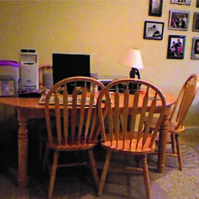
\includegraphics[width=\linewidth]{./Figures/nyu_depth_v2_img.jpg}
		\caption{}
	\end{subfigure}
	\begin{subfigure}[b]{0.24\linewidth}
	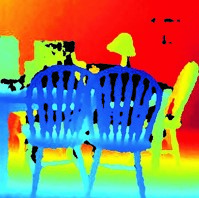
\includegraphics[width=\linewidth]{./Figures/nyu_depth_v2_depth.jpg}
	\caption{}
\end{subfigure}
	\begin{subfigure}[b]{0.24\linewidth}
	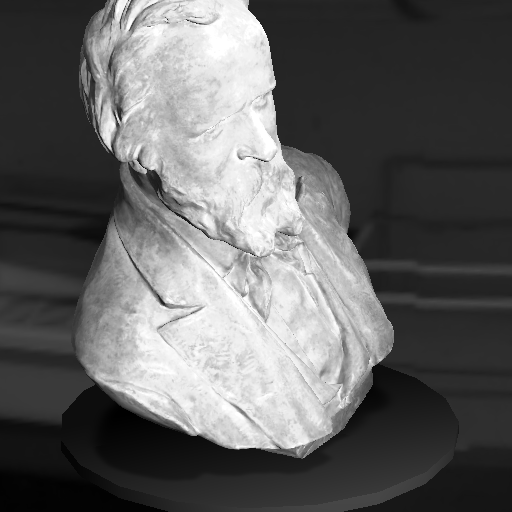
\includegraphics[width=\linewidth]{./Figures/train-image.png}
	\caption{}
\end{subfigure}
	\begin{subfigure}[b]{0.24\linewidth}
	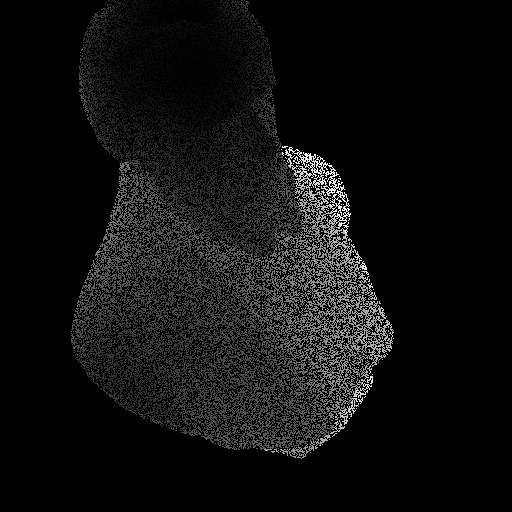
\includegraphics[width=\linewidth]{./Figures/train-depth-noise.png}
	\caption{}
\end{subfigure}
	\decoRule
	\caption{(a)-(b): Output from the RGB camera (a) and depth camera (b) of a scene in \textit{NYU Depth Dataset V2} \cite{nyu}. (c)-(d): Output from the gray-scale camera (c) and depth camera (d) of a scene in our proposed dataset \textit{synthetic-50-5}.}
	\label{fig:dataset-comparison}
\end{figure}
%% Photometric Stereo
Photometric stereo is another approach that derives the surface normal from the BRDF-based surface model. The surface normal is related to the observed intensity, the direction of incident light, the direction of outgoing light, and the light intensity. Several light conditions are required to obtain an optimal solution. \cite{CNN-PS} uses a CNN-based approach to learn the relationship between photometric stereo input and the surface normal under hundreds of lighting conditions, which is also robust to the effects of global illuminations. \cite{spline-net} is based on an illumination interpolation network to use only a sparse set of lights for photometric stereo tasks.


Our approach uses an RGB-D image but known light direction and calibrated information for surface normal inference, which considers multiple input data types into account for the estimation. 










